%%
%% This is file `sample-sigplan.tex',
%% generated with the docstrip utility.
%%
%% The original source files were:
%%
%% samples.dtx  (with options: `sigplan')
%% 
%% IMPORTANT NOTICE:
%% 
%% For the copyright see the source file.
%% 
%% Any modified versions of this file must be renamed
%% with new filenames distinct from sample-sigplan.tex.
%% 
%% For distribution of the original source see the terms
%% for copying and modification in the file samples.dtx.
%% 
%% This generated file may be distributed as long as the
%% original source files, as listed above, are part of the
%% same distribution. (The sources need not necessarily be
%% in the same archive or directory.)
%%
%% The first command in your LaTeX source must be the \documentclass command.
\documentclass[sigplan, screen,10pt]{acmart}
%% NOTE that a single column version is required for 
%% submission and peer review. This can be done by changing
%% the \doucmentclass[...]{acmart} in this template to 
%% \documentclass[manuscript,screen,review]{acmart}
%% 
%% To ensure 100% compatibility, please check the white list of
%% approved LaTeX packages to be used with the Master Article Template at
%% https://www.acm.org/publications/taps/whitelist-of-latex-packages 
%% before creating your document. The white list page provides 
%% information on how to submit additional LaTeX packages for 
%% review and adoption.
%% Fonts used in the template cannot be substituted; margin 
%% adjustments are not allowed.
%%
%% \BibTeX command to typeset BibTeX logo in the docs
\AtBeginDocument{%
  \providecommand\BibTeX{{%
    \normalfont B\kern-0.5em{\scshape i\kern-0.25em b}\kern-0.8em\TeX}}}

%% Rights management information.  This information is sent to you
%% when you complete the rights form.  These commands have SAMPLE
%% values in them; it is your responsibility as an author to replace
%% the commands and values with those provided to you when you
%% complete the rights form.

\usepackage{xcolor}
\usepackage{listings}
\usepackage{algpseudocode}
\usepackage{algorithm}
\usepackage{subcaption}
\usepackage{hyperref}
\usepackage{enumitem}
\usepackage{tabularx}

\usepackage{tikz}
\newcommand*\circled[1]{\tikz[baseline=(char.base)]{
            \node[shape=circle,draw,inner sep=2pt] (char) {#1};}}

\def\sectionautorefname{Sec.}
\def\tableautorefname{Tab.}
\def\figureautorefname{Fig.}
\def\subsectionautorefname{Sec.}
\def\algorithmautorefname{Algo.}


\definecolor{mGreen}{rgb}{0,0.6,0}
\definecolor{mGray}{rgb}{0.5,0.5,0.5}
\definecolor{mPurple}{rgb}{0.58,0,0.82}
\definecolor{backgroundColour}{rgb}{0.95,0.95,0.92}

% disable ~\cite{*} for now
\renewcommand{\cite}[1]{}


\lstdefinestyle{CStyle}{
    backgroundcolor=\color{backgroundColour},   
    commentstyle=\color{mGreen},
    keywordstyle=\color{magenta},
    numberstyle=\tiny\color{mGray},
    stringstyle=\color{mPurple},
    basicstyle=\footnotesize,
    breakatwhitespace=false,         
    breaklines=true,                 
    captionpos=b,                    
    keepspaces=true,                 
    numbers=left,                    
    numbersep=5pt,                  
    showspaces=false,                
    showstringspaces=false,
    showtabs=false,                  
    tabsize=2,
    language=C
}


\lstdefinestyle{customasm}{
    belowcaptionskip=1\baselineskip,
    frame=single, 
    frameround=tttt,
    xleftmargin=\parindent,
    language=[x86masm]Assembler,
    basicstyle=\footnotesize\ttfamily,
    commentstyle=\itshape\color{green!60!black},
    keywordstyle=\color{blue!80!black},
    identifierstyle=\color{red!80!black},
    tabsize=4,
    numbers=left,
    numbersep=8pt,
    stepnumber=1,
    numberstyle=\tiny\color{gray}, 
    columns = fullflexible,
}
%%
%% Submission ID.
%% Use this when submitting an article to a sponsored event. You'll
%% receive a unique submission ID from the organizers
%% of the event, and this ID should be used as the parameter to this command.
%%\acmSubmissionID{64}

%%
%% The majority of ACM publications use numbered citations and
%% references.  The command \citestyle{authoryear} switches to the
%% "author year" style.
%%
%% If you are preparing content for an event
%% sponsored by ACM SIGGRAPH, you must use the "author year" style of
%% citations and references.
%% Uncommenting
%% the next command will enable that style.
%%\citestyle{acmauthoryear}

%%
%% end of the preamble, start of the body of the document source.
\pagenumbering{arabic}
\begin{document}
\sloppy
%%
%% The "title" command has an optional parameter,
%% allowing the author to define a "short title" to be used in page headers.
\title{Decisions, decisions: Achieving near perfect page prefetching using decision trees}

%%
%% The "author" command and its associated commands are used to define
%% the authors and their affiliations.
%% Of note is the shared affiliation of the first two authors, and the
%% "authornote" and "authornotemark" commands
%% used to denote shared contribution to the research.
 \author{Shaurya Patel}
% \authornote{Both authors contributed equally to this research.}
%\email{spatel27@student.ubc.ca}
 \affiliation{%
   \institution{University of British Columbia}
 }

  \author{Tom Wang}
% \authornote{Both authors contributed equally to this research.}
%\email{siagraw@student.ubc.ca}
 \affiliation{%
   \institution{University of British Columbia}
 }

 

  \author{Joshua}
% \authornote{Both authors contributed equally to this research.}
%\email{siagraw@student.ubc.ca}
 \affiliation{%
   \institution{University of Waterloo}
 }

 \author{Margo Seltzer}
% \authornote{Both authors contributed equally to this research.}
%\email{mseltzer@cs.ubc.ca}
 \affiliation{%
   \institution{University of British Columbia}
 }
 
  \author{Alexandra Fedorova}
% \authornote{Both authors contributed equally to this research.}
%\email{sasha@ece.ubc.ca}
 \affiliation{%
   \institution{University of British Columbia}
 }

%%
%% By default, the full list of authors will be used in the page
%% headers. Often, this list is too long, and will overlap
%% other information printed in the page headers. This command allows
%% the author to define a more concise list
%% of authors' names for this purpose.
\renewcommand{\shortauthors}{Patel, et al.}

%%
%% The abstract is a short summary of the work to be presented in the
%% article.
\begin{abstract}

\end{abstract}

%%
%% Keywords. The author(s) should pick words that accurately describe
%% the work being presented. Separate the keywords with commas.



%%
%% This command processes the author and affiliation and title
%% information and builds the first part of the formatted document.
\settopmatter{printfolios=true}
% \maketitle

\section{Introduction}
% DRAM is a bottleneck in datacenters.
Increasing memory requirements for applications, e.g., machine learning, coupled with the slowdown of DRAM scaling~\cite{dram-1, dram-2}, makes DRAM one of the costliest components in data centers, constituting as much as 30\% of the entire cost~\cite{meta}. To accommodate increasing application memory demands without breaking the bank, operators often resort to far memory or memory disaggregation~\cite{aifm, canvas, dilos, fastswap, google, infiniswap, leap, memliner}. 
Far memory incorporates additional tiers of slower memory, such as NVM, SSDs, or software-based approaches, e.g., compressed swap~\cite{zswap-1, google, meta}. These tiers store memory pages that are less frequently accessed, freeing up costly DRAM for hot data.


% Current state of far memory systems in datacenters and their implementation.
There are various approaches to accessing far memory, such as application transparent approaches that use the swap subsystem~\cite{canvas, google, meta, fastswap, leap} or accessing far memory from userspace~\cite{aifm, hemem}. Regardless of the approach, accurate eviction and prefetching policies are essential to maintain application performance in the presence of far memory.
Leap demonstrated that effective memory page prefetching in the kernel increases application performance by up to $10 \times$~\cite{leap}. 
Kernel prefetchers similar to Leap rely on information collected during page faults to accurately predict strided accesses~\cite{vma-readahead, vm_fault_readahead, leap}. However, these prefetchers are ineffective at predicting irregular memory access patterns such as pointer-based accesses~\cite{CP, canvas, dilos}.

We propose a different approach of using Machine learning to do page prefetching.

Prior ML approaches for cache prefetching formulate the problem of predicting the next address to prefetch. We approach it differently, we formulate prefetching as a binary classification problem. 



\section{Background and Related work} \label{sec:2}

%\vspace{-0.45cm}
\subsection{Heuristic Page prefetching}
% Current state of Linux prefetchers
Page prefetchers are used in most modern operating systems to reduce the latency of page access from swap. 
Traditional algorithms prefetch based on sequential access to virtual addresses~\cite{vma-readahead, vm_fault_readahead} and are successful at fetching spatially related pages. 
One of the recent state of art prefetcher, Leap~\cite{leap}, improved traditional prefetching using majority trend detection to identify strided patterns; this makes Leap resilient to short-term irregularities in the memory access stream.
Leap improved performance for many applications but cannot prefetch irregular accesses. 
Multiple researchs have tried to improve Leap's performance by addressing its shortcomings~\cite{canvas, dilos, memliner} in \begin{itemize}
    \item prefetching irregular patterns,
    \item isolating the swap subsystem and memory access histories of threads, and
    \item coordinating memory accesses from the garbage collector and the application.
\end{itemize}

All the above resulted in the non-perfect prefetching performance of the prefetcher in our initial experiments.

\textbf{HOW TO CONTRAST OUR WORK WITH TRADITIONAL PREFETCHING?}

Studies~\cite{Aggressive} has shown the need for more aggressive prefetching to reduce the number of page faults while scrificing some protability and memory bandwidth. Thus, we propose a machine learning based prefetcher that can improve the prefetching accuracy and reduce the number of page faults.

\subsection{Machine Learning Prefetching}
Past success of machine learning in cache eviction~\cite{RelaxedBelady} and cache prefetching~\cite{LMAP} has shown that machine learning can be used to predict page accesses patterns with high accuracy.

\textbf{NEED MORE PREVIOUS WORKS}
% Previous work~\cite{LMAP} has shown that machine learning can be used to predict page accesses and prefetch pages with high accuracy.

\subsubsection{LSTM based prefetching}

LSTM, first introduced in 1997~\cite{LSTM}, is a type of recurrent neural network that is capable of learning long-term dependencies. An LSTM is composed of a cell $c$, a hidden state $h$, an input gate $i$, an output gate $o$, and a forget gate $f$. The cell remembers values over arbitrary time intervals and the three gates regulate the flow of information into and out of the cell. The hidden state $h$ is recurrent and is passed to the next time step. The process of an LSTM to process an input $x_t$ at time step $t$ is as follows:

\begin{enumerate}
    \item Parrellelly compute the input gate $i_t$, forget gate $f_t$, and output gate $o_t$.\begin{align*}
        i_t &= \sigma(W_{xi}x_t + W_{hi}h_{t-1} + W_{ci}c_{t-1} + b_i)\\
        f_t &= \sigma(W_{xf}x_t + W_{hf}h_{t-1} + W_{cf}c_{t-1} + b_f)\\
        o_t &= \sigma(W_{xo}x_t + W_{ho}h_{t-1} + W_{co}c_{t-1} + b_o)
    \end{align*}
    Here, $W$ and $b$ are the weights and biases of the gates, and $\sigma$ is the sigmoid function.
    \item Update the cell state $c_t$ and hidden state $h_t$.\begin{align*}
        c_t &= f_t \odot c_{t-1} + i_t \odot \tanh(W_{xc}x_t + W_{hc}h_{t-1} + b_c)\\
        h_t &= o_t \odot \tanh(c_t)
    \end{align*}
    Here, $\odot$ is the element-wise multiplication operator.
\end{enumerate}

LSTM has shown promising results in cache prefetching~\cite{LMAP} due to its ability to learn long-term dependencies. However, LSTM has a large number of parameters and is computationally expensive to train and run.

\subsubsection{Transformer based prefetching}

\textbf{CHECK OUT THIS PAPER}
\cite{Twilight}
\textbf{TO BE ADDED}

\subsubsection{Large Language Models based prefetching}

\textbf{TO BE ADDED}


\section{Motivation}\label{sec:3}

\textbf{WHAT MOTIVATES OUR WORK?}

Possible accessible virtual memory pages for a program is enonourmous. It is normal for program to access more than 1 GB of memory. Then that would be easy to get millions of possible pages the program will access. It is hard to predict which page the program will access next and to prefetch it before the program access it.

\subsection{Scope and Limitations}

\textbf{WHAT IS THE SCOPE OF OUR WORK?}

The scope of this work is to design a application-specific machine learning based page prefetcher that can predict the next page the program will access with high accuracy.

\textbf{WHAT ARE THE LIMITATIONS OF OUR WORK?}

\subsection{Information to be used for prefetching}

\textbf{WHAT INFORMATION CAN BE USED FOR PREFETCHING?}

There are lots of information that we can capture while a program is running. While collecting more information can help in predicting the next page the program will access, it can also increase the overhead of the prefetcher.

In this work, we will use the following information for prefetching:
\begin{enumerate}
    \item The virtual address of the page that caused the page fault.
    \item The program counter of the memory access instruction.
\end{enumerate}

These information are easily reachable and meaningful for prefetching.

\subsection{Prefeching as a classification problem}

Past work~\cite{LMAP} suggested that although page addresses are number, regression models are not suitable for prefetching. Instead, prefetching can be treated as a classification problem.

We treat the address space as a large, discrete vocabulary and perform classification. 

\textbf{DO WE TALK ABOUT OFFSET HERE?}

At the same time, the number of possible pages that can be accessed is very large. This makes the encoding of the page addresses as one-hot vectors very large. Also fixed encoding of the page addresses can be problematic as address randomization can change the encoding of the page addresses.

Privous work~\cite{LMAP} has suggested that offsets of page address accesses works better than absolute addresses, and since we are doing classification, we need to filter out the rare classes and only leave up to 50,000 most occured classes for offsets and pc values.

\begin{definition}
    {Offset} = {Next Page Address} - {Last Page address}
\end{definition}


%\begin{figure*}[t!]
%    \centering
%    \begin{subfigure}[t]{0.7\columnwidth}
%        \centering
%        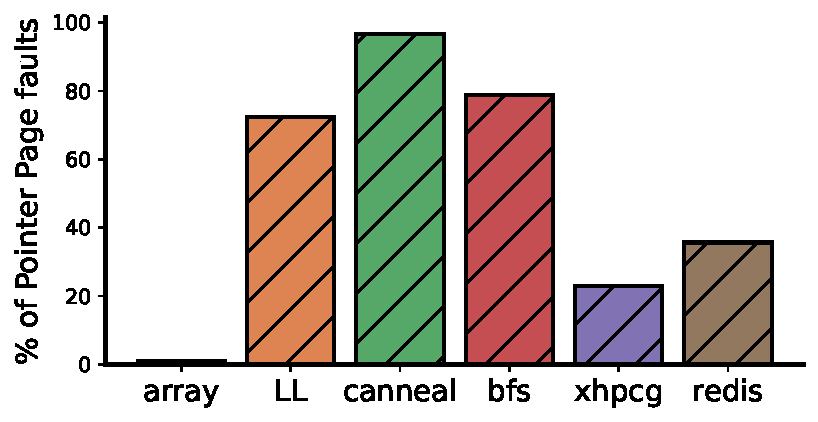
\includegraphics[height=2in]{images/bar_graph.pdf}
%        \caption{Percentage of pointer-based page faults for different workloads}
%        \label{fig:pointer_pagefaults}
%    \end{subfigure}%
%    ~ 
%    \begin{subfigure}[t]{0.7\columnwidth}
%        \centering
%        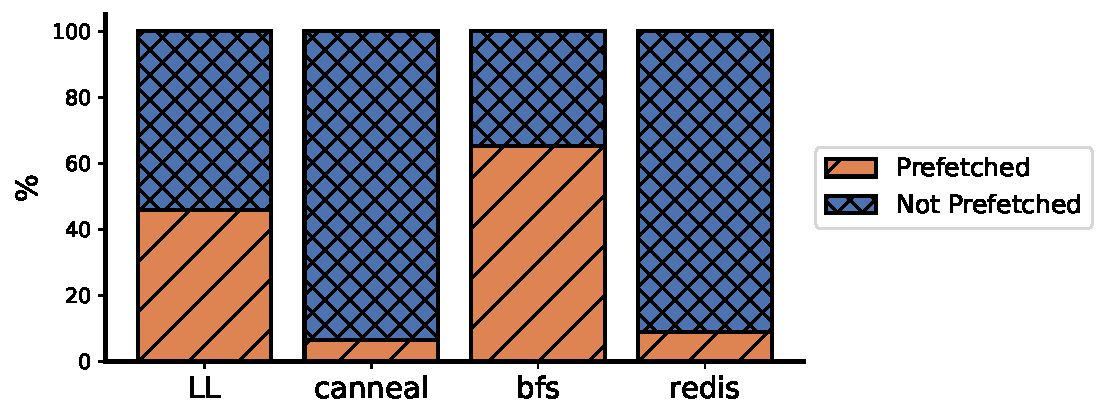
\includegraphics[height=2in]{images/divided_bar_graph.pdf}
%        \caption{Accuracy of the kernel prefetcher on pointer-based page faults.}
%        \label{fig:kernel_prefetcher_performance}
%    \end{subfigure}
    
%\end{figure*}

% To investigate which applications encounter pointer-based page faults, we developed a tool that analyzes a dynamic trace of register loads and page faults. We classify page faults into pointer-based and non-pointer-based and evaluate the performance of the default kernel prefetcher~\cite{vma-readahead}. Prior work performed a similar analysis to determine whether pointer chasing causes cache misses~\cite{cache-analysis}. However, the existence of pointer-chasing based cache misses does not guarantee the presence of pointer-based page faults. 
% For example, cache misses within a page do not cause page faults; only cache misses across pages might cause them. 
% Furthermore, page faults occur only when the application accesses swapped-out data.

% \subsection{Analyzer design} 
% Our analyzer merges two traces: a dynamic trace of all values loaded into registers and a trace of page fault addresses. A pointer is simply a memory location containing an address; without type information, it is impossible to distinguish a pointer from a non-pointer. 
% So, we borrow from prior work on cache prefetching~\cite{cache-analysis} to analyze dynamic application execution trace. If a value is loaded into a register from memory and is then used as an address or in an address computation, we consider it to be a pointer-based access. 
% For example, consider the linked list traversal and its corresponding assembly shown in \autoref{x86code}. 
% The value of \textit{curr} stored on the stack, is first loaded into register \texttt{rax} (Line 2) and subsequently accessed to load \textit{curr->next} from memory (Line 3). 
% %During the next node access, \textit{curr->next} will be accessed. 
% We classify this as a pointer-based access because the value of \textit{curr} was initially loaded into a register and subsequently used as an address. 
% If the access to \textit{curr} caused a page fault, we classify that page fault as a pointer-based page fault.

% \begin{comment}
% \begin{lstlisting}[caption={Linked list traversal example}, label={code:ll}, style=CStyle]
% struct node { ... struct node *next; }
% int main(void) {
%    ...
%    while(!curr) 
%         curr = curr->next;
%         // mov 0x2b46(%rip),%rax
%         // mov (%rax),%rax
%         // mov %rax,0x2b3c(%rip)
% }
% \end{lstlisting}
% \end{comment}

% \begin{lstlisting}[caption={x86 Assembly for traversal}, label=x86code,style=customasm,captionpos=b]
% ;curr = curr->next;
%  mov -0x600028(%rbp),%rax;load address of curr to rax
%  mov 0xff0(%rax),%rax;load the value of the curr->next
%  mov %rax,-0x600028(%rbp);store the loaded value
% \end{lstlisting}
    
% \vspace{-0.6cm}
% \subsection{Analyzer implementation}
% \begin{table}[]
% \resizebox{\columnwidth}{!}{%
% \renewcommand{\arraystretch}{1.4}
% \begin{tabular}{llc}

% \hline
% \textbf{Workload}           & \textbf{Source}    & \textbf{WSS}                 \\
% \hline
% Array streaming             & Microbenchmark    & 50\%                  \\
% Random linked list traversal (LL) & Microbenchmark    &      50\%            \\
% %Canneal                     & Parsec benchmark suite~\cite{parsec} &  50\%              \\
% %xHPCG                       & HPCG benchmark suite~\cite{hpcg}    &  50\%   \\
% Canneal                     & Parsec~\cite{parsec} &  50\%              \\
% xHPCG                       & HPCG~\cite{hpcg}    &  50\%   \\
% BFS on twitter dataset~\cite{twitter-dataset}      & GapBS~\cite{gapbs} & 25\%  \\
% %BFS on twitter dataset~\cite{twitter-dataset}      & GapBS~\cite{gapbs} (default processing system) & 25\%  \\

% Redis benchmark LRANGE      & Redis~\cite{redis} & 25\%       \\                    
% \hline
% \end{tabular}
% }

% \caption{Workloads used for analysis. 
% They represent a diverse spectrum of pointer-based fault intensity as shown in ~\autoref{fig:pointer_pagefaults}. WSS is the working set size in RAM}
% \label{tab:workloads}
% \vspace{-0.75cm}
% \end{table}

% We collect the dynamic trace of all values loaded into registers using Intel PIN (v3.26)~\cite{pin} and the page fault trace using \texttt{perf}~\cite{perf-probe} on Linux (v5.19). We run the analysis on Linux due to the availability of Intel PIN and \texttt{perf}, but we expect the analysis approach to generalize across platforms.
% We gather these traces during one program execution. We merge the two traces using timestamps and process them in sequential order. The analyzer maintains two data structures; the current state of the execution in a registers-to-value map and a set of loaded values. Once all the registers containing a particular value are overwritten, we remove the original value from the loaded values set. When a page fault occurs, the analyzer checks if the page address was loaded into a register by checking the currently loaded values set and then classifies the page fault as pointer-based if it is present. The analyzer can analyze traces in both offline and streaming mode.

% \subsection{Pointer-based page faults}
% \begin{figure}
% 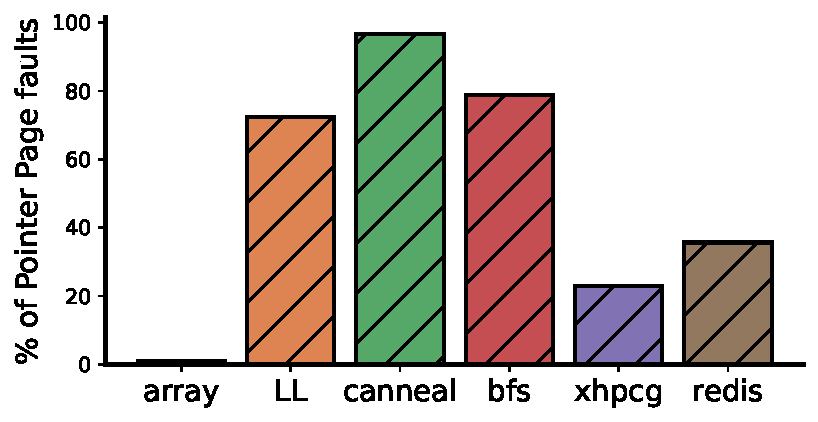
\includegraphics[height=3.3cm]{images/bar_graph.pdf}
% \caption{Percentage of pointer-based page faults for different workloads}
% \vspace{-0.25cm}
% \label{fig:pointer_pagefaults}
% %vspace{-1.3cm}
% \end{figure}

% \begin{figure}
% 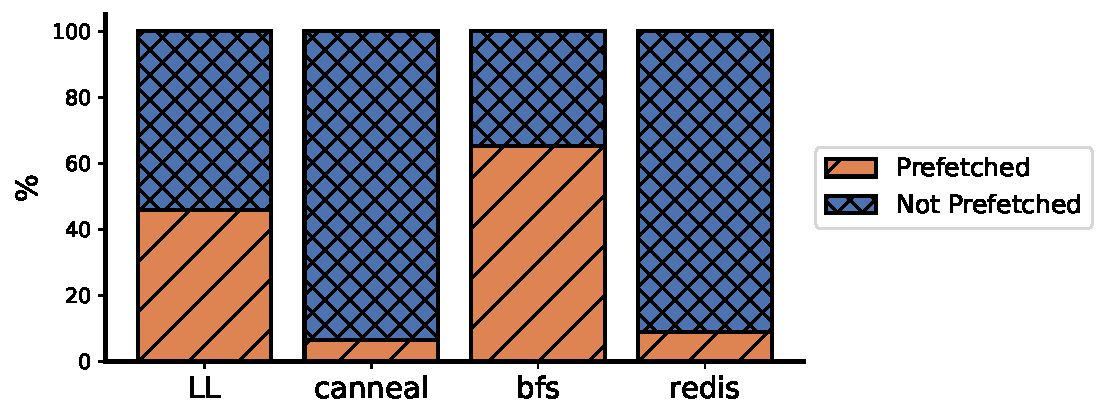
\includegraphics[height=3.3cm]{images/divided_bar_graph.pdf}
% \caption{Accuracy of the kernel prefetcher on pointer-based page faults.}
% \vspace{-0.25cm}
% \label{fig:kernel_prefetcher_performance}
% \end{figure}


% We analyzed different benchmarks (\autoref{tab:workloads}). In order to evaluate the potential of CHERI-picking in ideally suited workloads, we looked for benchmarks that demonstrate pointer-chasing behavior. We chose benchmarks based on prior work~\cite{classifying, dilos} having identified that they would benefit from pointer prefetching:
% Parsec's canneal~\cite{parsec}, xHPCG~\cite{hpcg} and Redis~\cite{redis}.
% %DiLOS~\cite{dilos} implemented an application-specific pointer prefetcher for Redis and showcased performance improvements; however, they did not analyze cache statistics. Hence, we replicated their approach. 
% To have confidence in the validity of our tool, we also designed a linked list traversal microbenchmark, which dynamically allocated page-sized nodes and ordered them randomly to render the kernel prefetcher ineffective. 
% For the array traversal microbenchmark, we allocated an array and streamed it sequentially twice. 
% To focus on page fault behavior, we constrained the program's memory using \texttt{cgroups}~\cite{cgroups}.

% \autoref{fig:pointer_pagefaults} presents our results. As we expect, a majority of the faults in the linked list microbenchmark are pointer-based, while none of the faults in the array streaming benchmark are. 
% Unsurprisingly, pointer-based page fault rates vary in other workloads, ranging from about 30\% for xHPCG 
% to almost 100\% for canneal. 
% Canneal accesses elements by indexing into two lists of pointers, so we expect it to have a majority of pointer-based faults. 
% The xHPCG benchmark maintains sparse vector objects and uses them to perform computation, leading to a lower percentage of pointer-based faults. The BFS benchmark performs breadth first search on a graph, stored in compressed sparse row format. Every access from a vertex to its children dereferences a pointer. 

% Our results suggest that some applications can benefit significantly from pointer prefetchers.
% An ideal pointer prefetcher should identify applications that can benefit from pointer prefetching without imposing overhead on applications that cannot, and achieve high prediction accuracy.



% \subsection{Performance of default kernel prefetcher on pointer-based page faults}

% The default kernel prefetchers detect sequential and strided accesses, make decisions quickly, and add little latency to the page fault path. Therefore pointer prefetchers should focus only on applications where the kernel prefetcher is ineffective. Figure \ref{fig:kernel_prefetcher_performance} illustrates the accuracy of the default kernel prefetcher~\cite{vma-readahead} on page faults that were classified as pointer-based. As expected, the results show that kernel prefetcher performance also varies, thus pointer prefetchers should be used to predict only those page faults that the default prefetcher misses. In the case of the linked list traversal, the kernel prefetcher predicts approximately 50\% of the pointer faults because the benchmark contains two loops; the first loop accesses the linked list nodes in the allocation order, while the second loop accesses them in random order. Accessing items
% in allocation order tends to produce a sequential access pattern that the default prefetcher handles well; accessing items in a random order produces an arbitrary pattern, so the default prefetcher fails. Surprisingly, although 78\% of page faults for BFS~\cite{gapbs} are classified as pointer-based, the kernel prefetcher successfully predicts 65\%, likely due to the compressed representation, which frequently places many child nodes on the same page. These applications leave limited room for improving prefetcher performance. In contrast, the kernel prefetcher predicts only about 8\% of the pointer-based faults in Redis, indicating significant potential. These findings emphasize that identifying applications where the default kernel prefetcher is ineffective is a key part of designing a pointer prefetcher.

% %Our analysis results show that important applications experience pointer-based faults and that the scope of pointer prefetchers for some applications is immense. An ideal pointer prefetcher should identify these applications without imposing a high overhead and achieve a high prediction accuracy on them.

\section{Design and Implementation} \label{sec:4}

In this section, we introduce the design and implementation of our LSTM, Transformer, and LLM based prefetchers. 


\subsection{LSTM based Prefetcher} \label{sec:4.1}

\begin{figure}[]
\centering
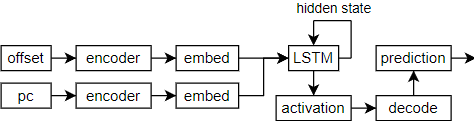
\includegraphics[width=\columnwidth]{images/LSTM.png}
\caption{LSTM based prefetcher architecture.}
\label{fig:lstm}
\Description{A diagram showing the architecture of an LSTM based prefetcher.}
\end{figure}

We implement an LSTM based prefetcher based on past work~\cite{LMAP}. It is shown at a high level in \autoref{fig:lstm}.

Each input offset, output offset and pc are encoded as a one hot representation of the total classes. Then the one hot encoding is embeded in a high dimensional space. The embeddings are then concatenated and fed to the LSTM. The LSTM outputs the probability of the next page to prefetch. To get multiple pages to prefetch, we can apply softmax on the output and sample from the distribution. 

\begin{itemize}
    \item Embeding dimension: 128
    \item LSTM hidden dimension: 128
    \item Number of LSTM layers: 2
\end{itemize}
% We begin by providing an overview of page fault handling in CheriBSD~\cite{cheribsd} to illustrate how CHERI-picking fits into the existing code. Traditional prefetchers rely on memory access history, which is accessible at page fault time, whereas CHERI-picking relies on the \emph{contents} of memory pages, which is available only after a page has been swapped in. This algorithmic difference produces a rather different implementation described in ~\autoref{sec:DI_CP_Policy}.

% \subsection{CheriBSD swap workflow}
% \label{sec:DI_swap}

% \begin{figure}[]
% \centering
% 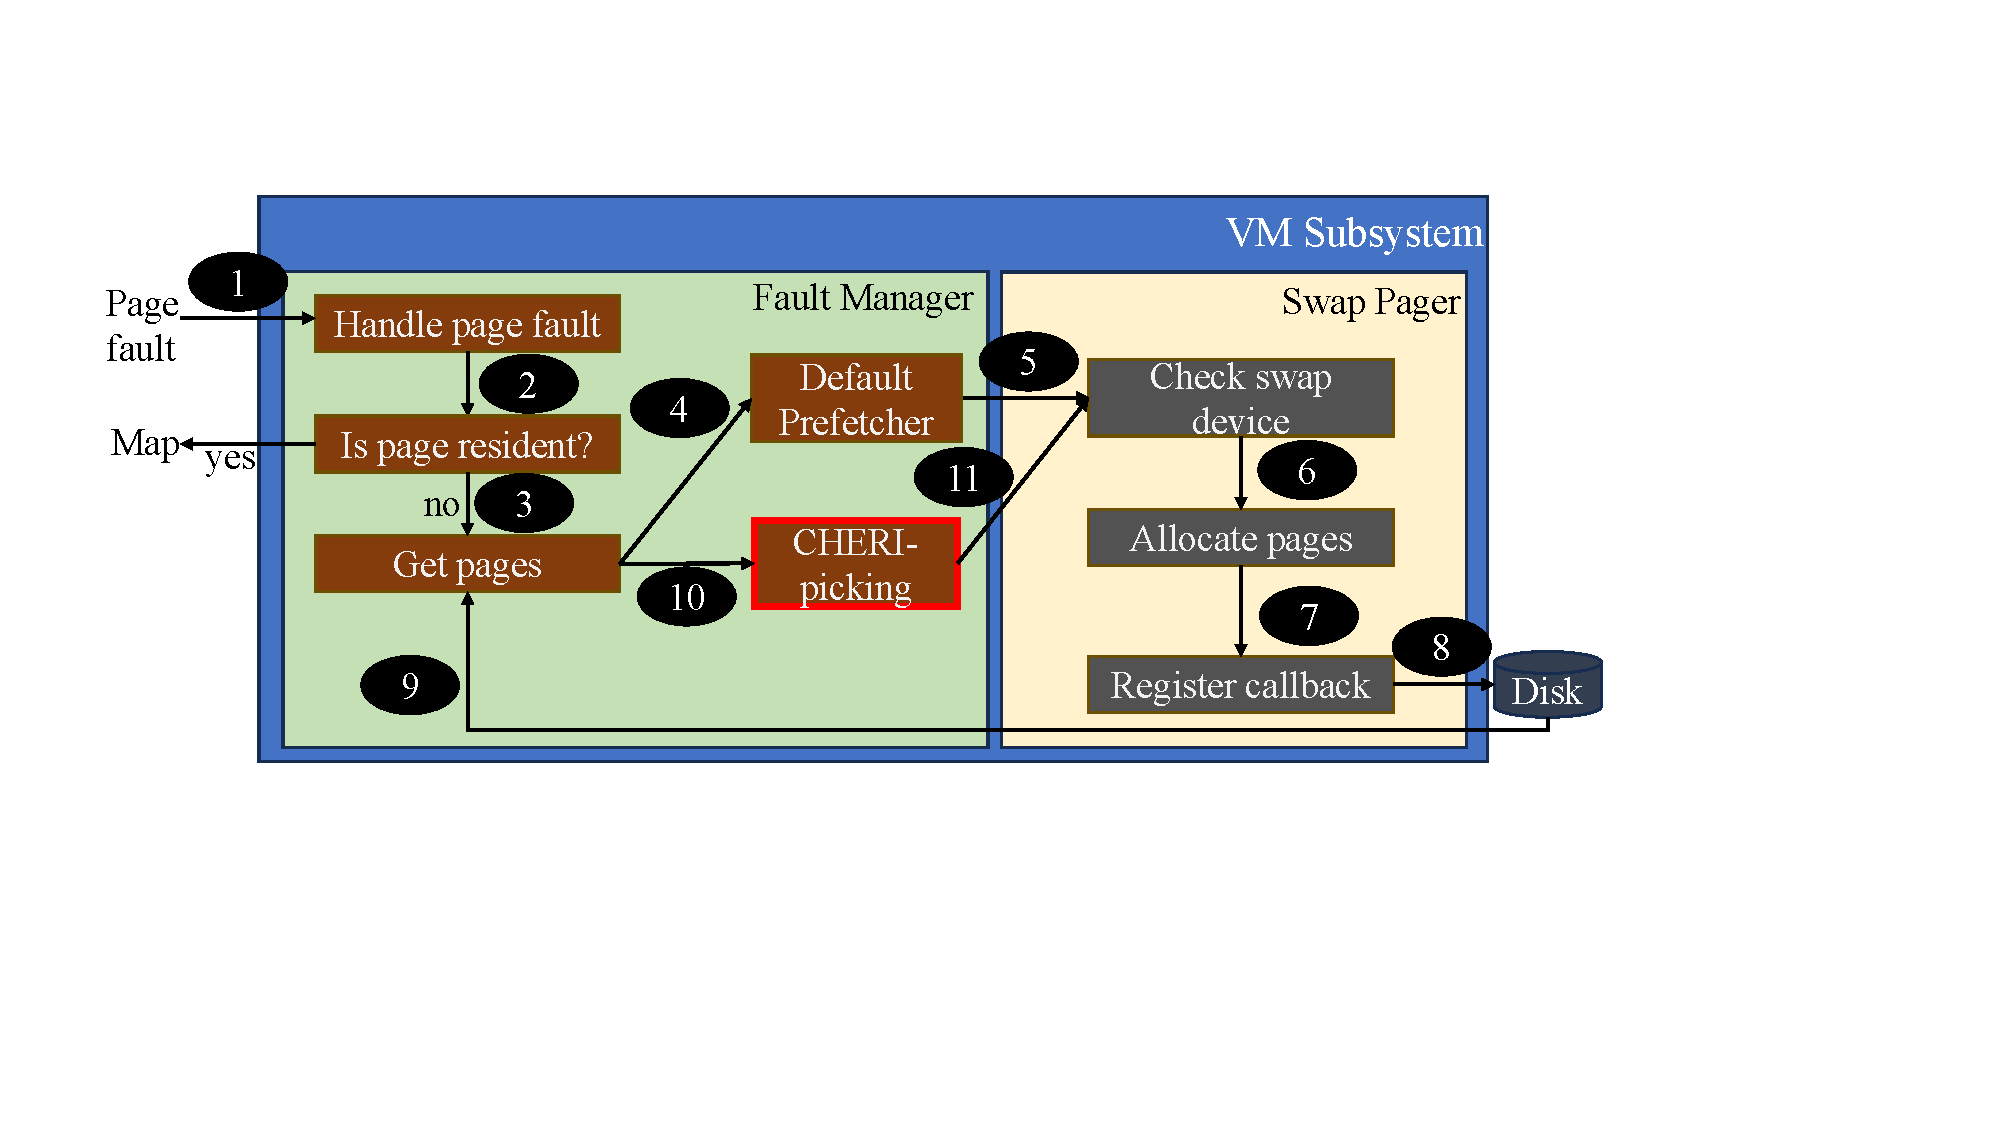
\includegraphics[width=\columnwidth]{images/CP_system_design_diagram.pdf}
% \caption{CheriBSD swap workflow. 
% CHERI-picking is invoked after the I/O request is completed.}
% \label{fig:system_design}
% \end{figure}

% % Link the image 
% % https://ubcca-my.sharepoint.com/:p:/g/personal/siagraw_student_ubc_ca/EWOPIZMY4VFIgUMZnJHmEu8B1EkDqDdvwLo2jrhZgjsXHQ?e=nWZW44
% \autoref{fig:system_design} illustrates the high-level design of the CheriBSD swapping workflow; the numbers in this section refer to the figure. 
% When a page fault occurs (\#1), the operating system checks if the page is already in memory (\#2). 
% If it is, CheriBSD maps the page into the application's address space and resumes application execution; this is known as a \textbf{soft fault}.

% If the page is not present in memory, the OS must retrieve the page from swap (in this case, the disk); this is called a \textbf{major fault}. The page fault dispatches a request to get pages (\#3). While getting the pages, the kernel executes the default prefetcher to detect sequential accesses (\#4). If the prefetcher detects a pattern, it checks if the requested page is present in the swap device (\#5). 
% If the requested page is in swap, it prepares for prefetching by allocating physical frames~ (\#6).
% It registers a callback for prefetched pages to put them into appropriate page queues when their I/O requests are completed (\#7).
% Then it finally issues an I/O request for the faulting page and any pages to be prefetched (\#8). 
% The swap manager returns after the faulting page is swapped in. 

% %Previous works~\cite{canvas, dilos} invoke application-level pointer prefetchers during page faults, and CHERI-picking also adopts this as the initial design choice. This approach provides the OS with insight into application execution and a starting point for making prefetch decisions.


% % After the faulting page is swapped in, the kernel invokes CHERI-picking. If, upon analyzing the page, the CHERI prefetcher discovers pointers to pages that are swapped out, it initiates their prefetching. Once the prefetcher completes these tasks, application execution resumes.

% % I removed this stuff from the design because this seems to be related work.
%  %CHERI-picking utilizes the contents of the faulted page to chase pointers, so we run it after the faulting page has been brought to memory. In the present design we do not  store pointer metadata of the swapped-out page separately from the page, so we must wait for the page to be swapped back in, so that we can find pointers
%  %However, recent work~\cite{leap} has demonstrated that batching can have a negative impact in a disaggregated environment.
%  %Application-level pointer prefetchers typically dispatch pointer requests to userspace when the kernel prefetcher either cannot make decisions or begins making faulty decisions.
%  % In those works, specialized prefetchers were developed inside the application to use application knowledge to chase pointers through memory. 
%  % The design of the CHERI-picking policy is similar to previous works~\cite{dilos, cache-analysis}.

% \subsection{CHERI-picking policy} 
% \label{sec:DI_CP_Policy}
% % This needs a bit more work if we want to explain that we create a new capability in the kernel to look at the page.
% CHERI-picking is highly configurable. We begin with an overview of when CHERI-picking is invoked, a description of the algorithm, and then discuss some key parameters available for tuning and future research. 
% CHERI-picking does not change the CheriBSD page fault path at all.
% Instead, after the callback for the faulting page occurs (\#9); CHERI-picking runs (\#10),
% %it scans the page, checking the capability on each address in the faulting page \circled{10}
% and according to configuration parameters, prefetches some pages (\#11)

% %Recall from ~\autoref{sec:2} that CHERI’s pure cap compilation mode ensures that every pointer in an application is tagged by the hardware and treated as a capability. Thus, CHERI-picking works only on applications compiled in purecap mode.



% \autoref{alg_1} describes the CHERI-picking algorithm. When the system swaps in a page, it obtains the kernel address for the physical page and iterates through its contents (lines 1-3). 
% %The prefetcher starts at the beginning of the page and examines the entire page for pointers. 
% For each address, CHERI-picking queries the hardware to retrieve the tag bit to determine if the address contains a pointer (line 4). 
% Upon finding a pointer, it confirms that the page is not already present in memory or prefetched (line 6-7). 
% It then verifies if the corresponding page is present in swap (line 8). 
% If the page is present in swap it is added to an asynchronous prefetch queue (line 9), and the swap manager fetches these pages into main memory. We prefetch a fixed number of pages, a parameter called \textit{prefetch\_count} (line 3), which can be tuned. We could limit ourselves to prefetching a small number of pages, pages whose pointers reside in certain ranges on the page, or addresses that meet any desired or learned criteria. CHERI-picking could also run on soft faults. We leave this kind of policy exploration for future work (\autoref{sec:6}).

% % OTHER POLICIES 
% % Which direction to explore? Currently, we only explore down the page, but exploring before the currently faulted address might be beneficial for some applications
% % Starting prefetching at the faulted addr rather than the top of the page is an obvious thing to explore 

% \begin{algorithm}
% \begin{algorithmic}[1]
% \Require $faulting\_page$, $prefetch\_count$
% \State $page\_addr \gets kernel\_addr(faulting\_page)$
% %\State $page\_end \gets page\_addr + page\_size$
% %\State $kernel\_capability \gets cheri\_setbounds(page\_addr, page\_size)$
% \While{$page\_addr < page\_addr + page\_size$ AND \\
%     \hspace{0.8cm} $ count < prefetch\_count \:$}
%     \State $is\_ptr \gets cheri\_gettag(*page\_addr)$
%     \If{$is\_ptr$} 
%         %\State $page\_allocated \gets lookup\_vm\_map()$
%         \If{$!page\_in\_ram()$ AND \\ 
%             \hspace{1.45cm}$!page\_prefetched()$}
%             \If{$page\_in\_swap()$}
%                 \State $get\_page\_async()$
%                 \State $count++$
%             \EndIf
%         \EndIf
%     \EndIf
%     \State $page\_addr~+= sizeof(CHERI\_Cap)$ \Comment{16 bytes}
% \EndWhile
% \end{algorithmic}
% \caption{CHERI-picking algorithm}\label{alg:cheri}
% \label{alg_1}
% \end{algorithm}

% \subsection{CHERI-picking design}
% \label{sec:DI_CP_design}
% We chose to implement CHERI-picking as a standalone function invoked by the callback to isolate our implementation during development and evaluation.
% This has several consequences and suggests directions for future work.

% Rather than implementing CHERI-picking in the swap callback function, one could merge CHERI-picking with the CheriBSD function 
% \texttt{swp\_pager\_meta\_cheri\_get\_tags()} that restores a page's capabilities~\cite{cheri_get_tags}.
% While we have not yet done that, this will likely reduce CHERI-picking's runtime overhead penalty, as discussed in
% ~\autoref{sec:overhead}.

% Recall from ~\autoref{sec:2} that CHERI’s purecap compilation mode ensures that every pointer in an application is tagged by the hardware and treated as a capability. Thus, CHERI-picking works only on applications compiled in purecap mode.

% As currently implemented, CHERI-picking always runs after the default prefetcher. 
% On one hand, CHERI-picking detects, and prefetches accesses that the default prefetcher cannot. 
% On the other hand, sometimes (as we’ll see in the microbenchmark results in ~\autoref{sec:5.1}), this can disrupt the performance of the default prefetcher.
% Better communication between the default prefetcher and CHERI-picking should be able to remedy this.


% \begin{comment}
% % Why we run cheripicking at major fault?
% % Why we run cheripicking after the page is swapped in?
% % What does cheri-picking run for?
% % % Why we run cheripicking at major fault?
% CHERI-picking doesn't change the code path at all. Instead, it runs when the callback for the faulting page occurs; it scans the page, checking the capability on each address in the faulting page, and according to configuration parameters, prefetches a selection of them. We implemented CP as a standalone module invoked by the callback to isolate our implementation during development and evaluation. This has several consequences and suggests directions for future work. 

% CHERI-picking makes prefetching decisions at major fault time. Prefetching at major fault time enables CHERI-picking to consider the context of application execution. We assume that spatial locality holds, indicating that pointers on the currently faulted page will likely be accessed soon. Further optimizations, such as prefetching at soft faults and performing pointer chasing in the kernel, are left as future work.

% % Why we run cheripicking after the page is swapped in?
% The default kernel prefetcher utilizes the memory access trace to make prefetching decisions. This trace is available prior to dispatching a request for the currently faulted page to disk, allowing for batching of sequential prefetching requests with the currently faulted page. In this situation, CHERI-picking distinguishes itself from the default prefetcher. In our current implementation, the request for the currently faulted page is sent to disk before CHERI-picking can execute the prefetcher. This is necessary as CHERI-picking needs to read the contents of the faulted page to find the pointers on the page. Currently, CHERI-picking always makes prefetching requests regardless of the default prefetchers decisions and requests pages that were potentially missed by the default prefetcher.

% % What does cheri-picking run for?
% CHERI-picking runs  for applications complied in \texttt{purecap} (see Section ~\ref{sec:2}) compilation mode, thus every pointer of an application is tagged by the hardware and treated as a capability. This allows CHERI-picking to run in an application-agnostic manner without the need for application hints.
% \end{comment}








% % TODO:
% %Explian: cheri_gettag, page_in_ram, page_in_swap

% \begin{comment}
% \textbf{CheriBSD Policy Implementation:} 
% To retrieve the tag from the metadata, $cheri\_gettag()$ utilizes a CHERI instruction. The prefetcher accesses CheriBSD's $vm\_map$, which contains a virtual address to $vm\_object$ mapping. Once the existence of the $vm\_object$ is confirmed, the prefetcher looks up the corresponding $pmap$, which maps $vm\_object$ to physical pages. The prefetcher sends prefetch requests to the swap pager, handling one page at a time. Although the prefetcher can batch multiple requests, our current focus is on increasing the VM cache hit rate. Optimizing disk accesses is left for future work.
% \end{comment}


\section{Evaluation}
\label{sec:5}

Correct prefetching choices can significantly reduce the number of page faults and improve the performance of applications. However, wrong prefetching choices can lead to unnecessary page faults due to memory pollusion and degrade performance. In this section, we evaluate the performance of the proposed ML prefetchers on a set of workloads and compare them with the state-of-the-art prefetcher, LEAP~\cite{leap}.

\subsection{Metrics}

We use memory access traces of benchmark workloads to evaluate the performance of the proposed ML prefetchers. The metrics we will focus on is:

\begin{definition}
    \text{Coverage} = $\frac{\text{Page faults predicted by Prefetching}}{\text{Total Page faults}}$
\end{definition}

\begin{definition}
    \text{Accuracy} = $\frac{\text{Page faults predicted by prefetching}}{\text{Total predictions}}$
\end{definition}

Coverage measures the percentage of page faults that were satisfied by the prefetcher. A higher coverage indicates that the prefetcher is able to predict more page faults. Accuracy measures the percentage of correct predictions made by the prefetcher. A higher accuracy indicates that the prefetcher is making correct predictions.

We want both coverage and accuracy to be high. However, there is a trade-off between the two. A prefetcher can achieve high coverage by prefetching aggressively, but this may lead to a decrease in accuracy. On the other hand, a prefetcher can achieve high accuracy by prefetching conservatively, but this may lead to a decrease in coverage. 

We focus on the coverage metric as it is more important for prefetchers in our experiment since none of our prefetchers are aggressive. \textbf{TODO: HOW TO WORD THIS BETTER?}

\subsection{Data Collection and processing}

To collecte page faults, we use \texttt{fltrace}~\cite{fltrace}, which will interpose on all \textbf{heap allocations}. Thus, we can collect page faults for all heap accesses. Stack accesses are excluded from the analysis since stack page faults are rare and are not the focus of this work.

Privous work~\cite{LMAP} has suggested that offsets of page address accesses works better than absolute addresses, and since we are doing classification, we need to filter out the rare classes and only leave up to 50,000 most occured classes for offsets and pc values.

\begin{definition}
    {Offset} = {Next Page Address} - {Last Page address}
\end{definition}

\texttt{fltrace} will need local RAM size to be set to run. It simulates the physical memory the program can access. Since each workload has a different memory requirement, we set the local RAM size to be 25\% and 50\% of the maximum memory requirement of the workload. This can be found by running \texttt{/usr/bin/time -v ./workload} and looking at the \texttt{Maximum resident set size}.

\subsection{Workloads}

We chose the following workloads for our evaluation:\begin{itemize}
    \item SPEC2017~\cite{SPEC2017}: mcf omnetpp and lbm with the default input files offered by the benchmark suite.
    \item GAP~\cite{gapbs}: the default \texttt{bfs, pr, bc} workloads on the \texttt{twitter} dataset~\cite{twitter-dataset}.
    \item WiredTiger~\cite{wiredtiger}: the default \texttt{ycsb-a} and \texttt{ycsb-c} workloads with \texttt{icount=30000000} in the benchmark configuration file.
    \item DiLos-redis~\cite{redis, dilos}: the \texttt{redis-benchmark} workload with \texttt{lrange} on a list of queries made by DiLOS~\cite{dilos}.
\end{itemize}

\subsection{Analysis}

\textbf{TODO: Wait for all my results to come in.}


% \begin{comment}
% %%%%%%%%%%%%%%%%%%%%%%%%%%%%%%%%%%%%%%%%%%%%%%%%%%%%%%%%%%%%%%%%%%%%%%%%%%%%%%%%%%%
% \begin{table}[hb!]
% \resizebox{\columnwidth}{!}{%
% \begin{tabular}{|l|c|c|}
% \hline
% \textbf{Workload}                & \textbf{Default} & \textbf{CHERI-picking} \\ \hline
% Sequential linked list traversal & 1,437K           & 1,018K                 \\ \hline
% Random linked list traversal     & 2K               & 1,044K                 \\ \hline
% \end{tabular}%
% }
% \caption{Soft faults on linked list microbenchmarks}
% \label{tab:microbenchmark_results}
% \end{table}
% %%%%%%%%%%%%%%%%%%%%%%%%%%%%%%%%%%%%%%%%%%%%%%%%%%%%%%%%%%%%%%%%%%%%%%%%%%%%%%%%%%%
% \end{comment}
% % Please add the following required packages to your document preamble:
% % \usepackage{multirow}
% \begin{table*}[]
% \begin{tabular}{|c|ccc|ccc|ccc|}
% \hline
% \multirow{{\textbf{Workload}} & \multicolumn{3}{c|}{\textbf{Soft faults (higher is better)}}                                     & \multicolumn{3}{c|}{\textbf{Major faults (lower is better)}}                                & \multicolumn{3}{c|}{\textbf{Coverage (higher is better)}}                                  \\ \cline{2-10} 
%                                    & \multicolumn{1}{c|}{\textbf{Default}} & \multicolumn{1}{c|}{\textbf{CP}} & \textbf{Change}      & \multicolumn{1}{c|}{\textbf{Default}} & \multicolumn{1}{c|}{\textbf{CP}} & \textbf{Change} & \multicolumn{1}{c|}{\textbf{Default}} & \multicolumn{1}{c|}{\textbf{CP}} & \textbf{Change} \\ \hline
%                                    \hline
% \textbf{Linked list sequential}                   & \multicolumn{1}{c|}{401K}             & \multicolumn{1}{c|}{227K}       & \textcolor{red}{$0.56\times$} & \multicolumn{1}{c|}{23K}           & \multicolumn{1}{c|}{224K}      & \textcolor{red}{$9.3\times$}     & \multicolumn{1}{c|}{94.5\%}           & \multicolumn{1}
% {c|}{50.2\%}     & \textcolor{red}{$0.53\times$}       \\ \hline
% \textbf{Linked list random}                   & \multicolumn{1}{c|}{11K}             & \multicolumn{1}{c|}{236K}       & $21.45\times$ & \multicolumn{1}{c|}{429K}           & \multicolumn{1}{c|}{235K}      & $0.54\times$    & \multicolumn{1}{c|}{2.07\%}           & \multicolumn{1}
% {c|}{50.12\%}     & $24.2\times$       \\ \hline \hline
% \textbf{canneal}                   & \multicolumn{1}{c|}{953K}             & \multicolumn{1}{c|}{3543K}       & $3.7\times$ & \multicolumn{1}{c|}{13.39M}           & \multicolumn{1}{c|}{14.57M}      & \textcolor{red}{$1.08\times$}
% & \multicolumn{1}{c|}{6.47\%}           & \multicolumn{1}{c|}{19.39\%}     & $3\times$       \\ \hline
% \textbf{BFS}                       & \multicolumn{1}{c|}{149K}             & \multicolumn{1}{c|}{204K}        & $1.35\times$         & \multicolumn{1}{c|}{92K}              & \multicolumn{1}{c|}{88K}         & $0.95\times$    & \multicolumn{1}{c|}{62.01\%}          & \multicolumn{1}{c|}{70.27\%}     & $1.13\times$    \\ \hline
% \end{tabular}%
% \caption{
% CHERI-picking (CP) improves the number of soft faults on standard benchmarks by up to $3.7\times$. 
% Values in red indicate instances where CP performs worse than the default prefetcher.
% }
% \label{tab:macrobenchmark-results}
% \end{table*}


% We assess CHERI-picking's performance on key prefetching metrics by comparing it to the default kernel prefetcher~\cite{vm_fault_readahead}. 
% We use a subset of the workloads we analyzed in ~\autoref{sec:3}. Specifically, we evaluate: the linked list microbenchmark, canneal on the native dataset, and BFS on the Wikipedia-links dataset~\cite{wikipedie-dataset}. We do not further analyze xHPCG as we saw that it is not pointer dense and has relatively few page faults ($\sim$50k). We also don't analyze the array traversal benchmark as the default prefetcher is expected to be effective. We leave further analysis of Redis as future work.

% We implemented CHERI-picking in the CheriBSD kernel version 22.12~\cite{cheribsd}, which delays mapping prefetched pages until they are accessed, unlike the default CheriBSD kernel, which proactively maps in prefetched pages.
% We run evaluations on an ARM Morello CHERI-capable processor~\cite{morelloarm} that contains 4 cores running at 2.4GHz. We limit memory so that the working set size of applications is twice that of the available memory, inducing memory pressure. 
% %We ported parsec's canneal~\cite{parsec} and GapBS~\cite{gapbs} to CheriBSD in \texttt{purecap} mode in under an hour.


% % Details:
% \begin{comment}
% CheriBSD    : 22.12 
% ARM Version : Armv8-A architecture version Armv8.2-A.
% n-cores     : 4
% clock rate  : 2.4 GHz (system Main clock)
% cache config: (below)
% Two dual-core Rainier clusters. Each cluster has:
% ◦ 64KB private L1 instruction cache for each core
% ◦ 64KB private L1 data cache for each core
% ◦ 1MB private L2 unified cache for each core
% ◦ 1MB shared L3 unified cache in the DynamIQ™ Shared Unit (DSU) Flash Cache Module
% (FCM)

% \end{comment}






% We evaluate prefetching performance using the following metrics:
% %\vspace{-0.2cm}
% \begin{itemize}[wide, labelindent=3pt]
%     \item \textbf{Soft faults:} These page faults occur when a page is already in memory, but not mapped into an application's address space;
%     indicating the prefetcher's prediction capacity. 
%     \item \textbf{Major faults:} These page faults occur when the page is not present in memory and indicate the faults not predicted by the prefetcher, encompassing mandatory misses and prefetcher miss predictions. 
%     \item \textbf{Coverage:} The percentage of page faults that were satisfied by previously prefetched pages.
%     %CHERI-picking.
% \end{itemize}
% In ~\autoref{sec:6}, we discuss CHERI-picking performance overhead and challenges.

% %%%%%%%%%%%%%%%%%%%%%%%%%%%%%%%%%%%%%%%%%%%%%%%%%%%%%%%%%%%%%%%%%%%%%%%%%%%%%%%%%%%
% \begin{comment}
% \begin{table}[]
% \resizebox{\columnwidth}{!}{%
% \begin{tabular}{|l|l|}

% \hline
% \textbf{Workload}           & \textbf{System}                \\
% \hline
% Random Linked list traversal & Microbenchmark          \\
% \hline
% Sequential Linked list traversal          & Microbenchmark                  \\
% \hline
% Canneal on native dataset                     & Parsec benchmark suite~\cite{parsec}           \\
% \hline
% BFS on wikipedia-links dataset~\cite{wikipedie-dataset}      & GapBS~\cite{gapbs} (default processing system)  \\
% \hline
% \end{tabular}
% }
% \caption{Workloads and benchmarks used for evaluation}
% \label{tab:evaluation_workloads}
% \end{table}
% \end{comment}
% %%%%%%%%%%%%%%%%%%%%%%%%%%%%%%%%%%%%%%%%%%%%%%%%%%%%%%%%%%%%%%%%%%%%%%%%%%%%%%%%%%%

% %\vspace{-0.2cm}
% \subsection{Microbenchmark results}
% \label{sec:5.1}

% \begin{comment}
% We use two different versions of the linked list microbenchmark from ~\autoref{sec:3}. In one, we traverse the list in allocation order, and in the other, we traverse the elements in random order. 
% Each node of the linked list is a page size. We allocate a total of 500k pages (equal to 2GB).
% When the linked list is traversed in allocation order, the page access order is sequential as well, due to continuous allocations. 
% We expect that the default prefetcher is effective for this workload and the results in ~\autoref{tab:macrobenchmark-results} confirm this. 
% However, since each page access is a pointer-based access, CHERI-picking also runs.
% %CHERI-picking's predictions interfere with the default prefetcher's semantics.
% At a major fault, CHERI-picking predicts the next node of the linked list.
% This prediction disrupts the default prefetcher's expectation of two sequential major faults, as the default prefetcher needs two faults to ensure that a sequential pattern exists.
% Additionally, because the page accesses are sequential, the default prefetcher can prefetch 16 pages at each major fault. CHERI-picking only prefetches one pointer that is present on the currently faulted linked list node.
% This interference issue could be resolved by combining the two prefetching algorithms.


% In the case of linked list traversal in random order, CHERI-picking outperforms the default prefetcher by predicting faults using pointers, because CHERI-picking runs at major faults, it will predict the next node for the currently faulted node, but it won't prefetch in-depth, thus the node following the prefetched node will again cause a major fault. On the other hand, the default prefetcher fails to predict any of the faults. 
% This scenario can be reproduced in various pointer-chasing workloads where the allocation and access order of data structures differ and when datastructures are randomly accessed.
% \end{comment}

% We use two different versions of the linked list microbenchmark from ~\autoref{sec:3}. In one version, we traverse the list in allocation order, while in the other, we traverse the elements in random order. We allocate a total of 500k pages (equal to 2GB). When we order the pages in allocation order (sequential), the default prefetcher proves effective, as demonstrated in ~\autoref{tab:macrobenchmark-results}. The default prefetcher's initial prediction requires two sequential major faults to detect a sequential pattern. 
% \begin{comment}
% Afterward, it prefetches a set number of pages and continues to prefetch pages accurately for each subsequent major fault. 
% However, since we currently do not communicate any information between the default prefetcher and CHERI-picking, CHERI-picking also runs on each page and predicts just one page (the next one in the list) to prefetch.
% This means that the two sequential major faults that the default prefetcher needs to detect sequential access never happen.
% Thus, CHERI-picking actually makes things worse!
% Additionally, since CHERI-picking does not run on soft faults (yet), this benchmarks requires one hard fault for each prefetch, so CHERI-picking prefetches only 50\% of the faults.
% \end{comment}
% However, CHERI-picking, which also prefetches pages here due to pointer-chasing, eliminates the second major fault and prevents the default prefetcher from detecting the sequential pattern. Further, CHERI-picking is worse than the default prefetcher here, because it prefetches one page at a time (in the current prototype), while the default prefetcher could fetch several (minimum 7 pages).
% This interference issue could be resolved by combining the two prefetching algorithms or communicating between them.

% When we order the pages randomly, CHERI-picking works as expected and outperforms the default prefetcher; as we saw above, it still prefetches only 50\% of the faulting pages, due to its not running at soft fault time. Given the random order of page accesses, the default prefetcher fails to predict any of the faults.
% This scenario can be present in various pointer-chasing workloads where the data structure's allocation and access order 
% differ.

% \subsection{Standard Benchmarks}
% We next ran the BFS and canneal benchmarks described in ~\autoref{sec:3}. We set the \texttt{prefetch\_count} to four pages for these tests as analysis indicates that these benchmarks are pointer-dense.

% The default prefetcher predicts 900k faults for the canneal benchmark, 6.47\% of the total page faults.
% CHERI-picking predicts 3M faults, covering 19.39\%, and improving upon the default prefetcher by $3\times$. The canneal benchmark maintains a list of elements, with each element containing two lists of pointers to other elements in the elements list. 
% The benchmark first randomly indexes into the elements list to select an element and then traverses through every element in the two lists within the selected element.
% The randomness in indexing the first element makes it challenging to prefetch. 
% However, CHERI-picking can predict the pointers accessed by the two lists inside the element, leading to an increase in soft faults and coverage compared to the default prefetcher.

% The default prefetcher worked well for BFS, based on the results from ~\autoref{fig:kernel_prefetcher_performance}. 
% CHERI-picking improves coverage by $13\%$ over the default prefetcher, demonstrating that pointer prefetchers can improve coverage for BFS, albeit only by a small amount.

% \subsection{CHERI-picking overhead}
% \label{sec:overhead}
% %The astute reader will have noticed that so far, we have focused only on the accuracy of the prefetcher and artfully side-stepped performance issues. 
% Currently, CHERI-picking has two major sources of overhead. First, when we traverse the page looking for pointers, this adds latency to the page fault. Second, when we don't prefetch the page early enough (timeliness), it leads to blocking soft faults. 
% The execution time of the sequential linked list microbenchmark with
% CHERI-picking is twice that of the default prefetcher because
% CHERI-picking adds about $7\mu$s to every page fault (which is clearly unacceptable)
% and also disrupts the default kernel prefetcher (\autoref{sec:5.1}).
% The execution time of the random linked list microbenchmark is the same for both prefetchers.
% Even though this is a pointer-chasing workload, we do not see a performance boost, because
% CHERI-picking also causes many blocking soft faults, which occur when a prefetched page is still in transit from disk. In part, this is due to the nature of our microbenchmark; we do not process the nodes on the list at all. In reality, there will be some processing on each node in the list, which could mitigate these blocking faults.
% In canneal, for example, only 13\% of soft faults block.



\vspace{-0.2cm}
\section{Challenges and Future work} 
\label{sec:6}

Our focus in CHERI-picking was to demonstrate the feasibility of a generalized kernel pointer prefetcher. However, the prototype is not yet a complete implementation. While CHERI-picking improves coverage for BFS and canneal, it does not reduce the number of major faults for canneal; Canneal is a pointer-dense benchmark and a challenging one for CHERI-picking.
Each faulted page contains many pointers; canneal first indexes into a pointer array randomly. 
If that access causes a page fault, CHERI-picking will prefetch 4 pages that will not be used.
In fact, CHERI-picking prefetches 30 million pages, but only about 10\% of those are ever accessed.
BFS provides a nice contrast here; although it too is pointer dense, since we are traversing the entire data structure, every pointer prefetched is ultimately accessed. This results in 5\% fewer major faults compared to the default prefetcher. Optimizing the CHERI-picking policy parameters such as \texttt{prefetch\_count} is critical to reduce thrashing. 

%We must be cautious when selecting the backend device, considering the overheads in CHERI-picking and the fact that it only executes after swapping in the faulted page. The cost of scanning a page might still be lower than slower backend devices like disks and SSDs. However, the scanning cost might be a bottleneck for faster far memory devices like CXL-attached memory or RDMA. To address this, we plan to leverage existing swap data structures maintained by CheriBSD~\cite{cheribsd} and investigate executing the CHERI-picking algorithm asynchronously.  Additionally, potential future hardware-based optimizations for scanning processes can help remove the overhead.

There are several avenues of performance optimization that we intend to investigate to address the overheads of CHERI-picking. First, we need to add better communication between the swap system, the default prefetcher, and CHERI-picking; by re-using swap data structures, we can optimize the CHERI-picking policy and record sufficient metadata to prevent CHERI-picking from running for cases when the default prefetcher is effective.
Second, we do not run CHERI-picking on soft-faulting pages, but doing so asynchronously provides for more aggressive prefetching.
Third, blindly prefetching a fixed number of pages on every faulted-in page is unlikely to be a good strategy; we need to explore how to better identify the right pointers to prefetch. Fourth, optimizing the I/O requests that CHERI-picking issues is essential; along with examining CHERI-picking performance on other swap backends such as RDMA. The overhead of scanning pages might be a bottleneck for faster swap backends such as CXL-attached memory or RDMA. To maintain performance in these scenarios, investigating techniques such as asynchronous execution of the CHERI-picking algorithm will be critical.  Additionally, potential future hardware optimizations such as scanning the tags in hardware while copying a page can help remove the overhead.
%Fourth, optimizing our I/O stack and using a faster swap backend, such as RDMA with CHERI-picking, will reduce blocking faults and improve performance.

%CHERI-picking results in numerous blocking soft faults, these are faults occurring on a page that was prefetched but is still in transit from disk. 
%\textcolor{red}{add a line about how to handle processes that may not have CHERI caps.}
%While not all faults are blocking soft faults (e.g., canneal experiences 400K blocked soft faults, accounting for 13\% of soft faults), further enhancing the policy and analyzing the application are crucial steps to improve the system and achieve lower execution time. 
%We will continue with the analysis and optimization of our implementation to demonstrate improvements in real workloads such as Redis.


%\vspace{-0.5cm}
\section{Conclusion} 

CHERI-picking represents an initial step towards integrating application-specific prefetchers in the kernel.
Our analysis reveals that both applications and benchmarks exhibit pointer-chasing patterns that the default kernel prefetcher fails to predict effectively. 
Through evaluation, we demonstrate benchmarks where the kernel prefetcher's effectiveness is limited, while CHERI-picking successfully predicts future accesses. 
CHERI-picking significantly enhances coverage for two standard benchmarks, improving it by up to a factor of three. 
However, much remains to be done to transform our prototype into a practical reality.

\section*{Acknowledgments}
The authors would like to thank --  Robert Watson for access to Morello hardware; George Neville-Neil, Jessica Clarke, Brooke Davis, John Baldwin, and Mark Johnston for their help with CheriBSD; Reto Achermann, Joel Nider, and the anonymous reviewers of PLOS for their feedback on the draft. We acknowledge the support of the Natural Sciences and Engineering Research Council of Canada (NSERC).
%Although the results highlight the effectiveness of CHERI-picking, further work is necessary to enhance its performance with real workloads. CHERI-picking must address the problem of predicting pointers quickly to improve performance and prefetch pointers before they are actually accessed. This has been discussed in previous research on caching~\cite{cache-analysis, cache-mowry-pointer}. If the work done between two pointer accesses is not sufficiently long, the prefetcher may not achieve significant savings. We encountered a similar issue during the linked list traversal. However, page prefetchers have the advantage of prefetching multiple pointers as a page can accommodate numerous pointers. This distinction sets page prefetchers apart from cache prefetchers.

%While we built upon existing prefetchers and chose to execute CHERI-picking during major faults, additional analysis is required to determine when to invoke CHERI-picking. This decision plays a crucial role in enhancing the potential to prefetch pointers before they are accessed and improving the prefetcher's accuracy. One approach is to also run CHERI-picking during soft faults, as traditional prefetchers do not benefit from such instances, whereas CHERI-picking can. Furthermore, it is essential to explore tunable parameters that can significantly impact the overhead of CHERI-picking. These parameters include determining the number of pointers to prefetch from a single page, the depth of exploration, and the direction of prefetching. By investigating these aspects, we can better understand and optimize CHERI-picking.

%CHERI-picking serves as a foundation for integrating pointer prefetchers within the kernel. However, further analysis and exploration are necessary to transform pointer prefetchers into a practical reality.


%%
%% The next two lines define the bibliography style to be used, and
%% the bibliography file.
% \bibliographystyle{ACM-Reference-Format}
% \bibliography{sample-base}
\end{document}
\endinput
%%
%% End of file `sample-sigplan.tex'.
